\documentclass[AMS,STIX2COL]{WileyNJD-v2}
\usepackage{lineno,hyperref}
\usepackage{subcaption}
\usepackage{amsmath,amssymb,amsfonts}
\articletype{Article Type}%

\received{26 April 2016}
\revised{6 June 2016}
\accepted{6 June 2016}
dfghjdkjfhgdjkfhgjkgfdh
\raggedbottom

\begin{document}

\title{Application of Grey System Theory to Phosphorite Sinter Process: From Modeling to Control.}

\author[1]{Nigina Toktassynova}

\author[2]{Hassen Fourati}

\author[1]{Batyrbek Suleimenov}

\authormark{N. Toktassynova \textsc{et al}}


\address[1]{\orgdiv{Automation and control}, \orgname{Satbayev University}, \orgaddress{\state{050013 Almaty}, \country{Kazakhstan}}}

\address[2]{\orgdiv{GIPSA-Lab}, \orgname{University Grenoble Alpes}, \orgaddress{\state{38000 Grenoble}, \country{France}}}

\corres{*Hassen Fourati. \email{hassen.fourati@gipsa-lab.fr}}

\presentaddress{This is sample for present address text this is sample for present address text}

\abstract[Summary]{The sintering process of phosphorite ore occurs with a large amount of return caused by untimely process control. The control task of the phosphorite ore sintering is to regulate parameters of the process to obtain a high quality sinter. The parameter clearly responsible on the sinter quality is the temperature in the wind box. Therefore, in order to solve the control task, it is necessary to predict the highest temperature of the charge (called also burn through point (BTP)). 
In this paper, the theory of grey systems is used as a predictive model, which makes it possible to obtain an adequate model that uses a small number of initial samples of real temperature data. Based on the grey model GMC(1,n) a new optimal model was presented, which is constructed by using optimization algorithm. Optimal model predicts the BTP, and to find out an optimal regulation, a control synthesis is carried out through an optimization of the prediction according to the “particle swarm” algorithm.}

\keywords{burn through point, control structure, grey system, optimization algorithm, predictive model, sinter process}

\jnlcitation{\cname{%
\author{Toktassynova N.}, 
\author{Fourati H.}, 
\author{Suleimenov B.}, 
} (\cyear{2020}), 
\ctitle{Modeling and Control Approach of a Phosphorite Sinter Process with Grey System Theory}, \cjournal{Asian Journal of Control}, \cvol{2020;00:1--6}.}

\maketitle

\footnotetext{\textbf{Abbreviations:} BTP, burn through point; GMC, convolution grey model}


\section{Introduction}\label{sec1}
Sintering in metallurgy is a thermal process that occurs in a metallurgical charge, composed of ore pellets, concentrates and fuel (coke). The technological process is shown in Fig.~\ref{fig:SinterProcess}, it begins with the preparation of the phosphorus ore in the predetermined proportions, which includes the following components: phosphorus trifle, coke trifle and secondary return. This return represents the bad quality sinter after breaking in yellow phosphorus production. Next, the phosphorus ore is mixed with a cold return and other components in a special drum to form the charge. This latter is loaded onto the moving grate of the sintering machine and is ignited using natural gas or $CO_2$ under the horn. With the help of wind boxes under the grate, an underpressure is created and a stream of hot gases gradually passes through the layer of 260 mm in height from the top to the underlying layers, ensuring the burning of coke breeze particles and the formation of sinter. At the end of sintering machine, the sinter is cooled and crushed, and the poorly sintered charge is sent to the beginning of the process. 

\begin{figure}[htbp]
	\centering
	\resizebox*{9 cm}{!}{
		\includegraphics{1}}
	\caption{Technological chain of sintering process.} \label{fig:SinterProcess}
\end{figure}

Due to the process non-linearity, the real time quality control is a complex task. In practice, the operator makes changes to the process after the product is obtained, which leads to a large quantity of return and expenses for re-sintering. In this regard, it becomes necessary to predict the sinter quality in advance and control the process based on a predictive model.
One of the key indicators of the sintering quality is the BTP that indicates the sintering process completion and represents the point with the highest temperature. The problem of BTP prediction and control is studied in a lot of works using various algorithms such as neural networks (NN), genetic algorithms, cluster analysis and fuzzy control. Due to the evolution and widespread of NN, a large number of works related to prediction, use this method in the BTP prediction and control. For example in \cite{Feng2000}, the mathematics inflexion point of waste gas temperature curve in the middle of the strand was measured at different times (600 groups of data) and fed to the input of a multilayer NN, whose output predicts the BTP values by 5 steps forward. NN is used in \cite{LiPeng2006}, where the strand speed and BTP at the previous instants of time were given to the network inputs. The network, together with the training algorithm, served to update the BTP model. In \cite{Du2017} the current value of BTP, temperatures in the middle, in the end of the process and the strand speed were given to the input of a NN to predict the BTP and an intelligent control of the iron ore sintering process was proposed. A fuzzy NN was used in the BTP prediction \cite{Wang20141}. Temperatures in wind boxes were chosen as inputs and the BTP temperature as output of model.

\footnotetext{\textbf{Abbreviations:} NN, neural network}

Other works \cite{Wu2006}, \cite{Wu2012} use two BTP predictive models: temporary and technological. Then, to predict the permeability of lead-zinc ore in \cite{Wu2006} the temporary NN was supplied with 6 previous values for permeability, and the technological NN used the temperature of fire, humidity, sulfur, lead, silicon dioxide content and strand speed. In \cite{Wu2012}, the BTP grey model GM(1,1) of lead-zinc ore was applied, and the charge permeability and strand speed of the pallets were fed to the technological neural network input. The approach proposed in \cite{Wu2012b} for BTP prediction of iron ore sintering used the integration of grey model and NN. Here the result of the grey model GM(1,1), especially the gas temperature in wind boxes, is one of the inputs of the back propagation NN, along with the strand speed and BTP at current time. The three works, with two predictive models, used a fuzzy expert controller that maintains the BTP desired position within the specified boundaries.

In \cite{Du2019}, carbon efficiency optimization model and BTP expert-fuzzy controller were presented. The main idea is to improve the carbon efficiency by using intelligent integrated control strategy for the BTP. Strand velocity of carbon efficiency optimization model and BTP expert-fuzzy controller are integrated by fuzzy satisfaction degree method, which calculates the end strand velocity.
BTP prediction model developed in \cite{Chen2017} also used 2 models.
Temperatures in wind boxes are supplied to a BTP soft-sensor model (1st model) to predict the BTP position. BTP temperature prediction model (2nd model) used BTP temperatures, which were obtained in previous steps. The outputs of 2 models  together with strand velocity are used as inputs of fuzzy robust control, which is based on an improved Takagi–Sugeno model.

From other side, genetic algorithms are used within this framework. Thus, in \cite{Wu-ShanCheng2005} an adaptive genetic algorithm was used to control BTP in iron ore sintering process, where the input layer of the NN is parameters of the initial material, density, strand speed and ignition temperature, and the output layer is the values of temperature and underpressure of sintering gases and gases in wind boxes. The genetic NN was used also for the BTP prediction of iron ore sintering in \cite{Cheng2006}, where 707 groups of data were given to the input after clustering and classification of temperature and underpressure vectors from 18 wind boxes. The adaptive structural clustering system is based on a spatial clustering of initial data, a self-organizing NN map for extracting data relevancy properties and a Kohonen map for learning network. The idea of clustering was used in \cite{Shang2010} for the BTP prediction model of iron ore sintering. The K-means clustering module, whose inputs are the cold-charge permeability model, the ignition temperature and the coke residue values, was used to form clusters. The predictive model based on the clusters from K-means module were fed to the dynamic model of temperature and underpressure, which is constructed using the novel genetic programming. A firework algorithm based on genetic algorithm was proposed in \cite{Wang2018} to optimize the sintering terminal prediction model of support vector machine. Seven main parameters were used as input to predict the BTP.

Models that do not use the NN for BTP prediction are based on equations of temperature or BTP. For example, in \cite{Kwon1999}, the predicted value of the BTP was determined by the least squares method based on the historical data and, depending on the signal of the event based model which determines the time until the end of the  movement. The event based model of BTP in iron ore sintering is represented by a linear time-constant discrete model. 
In \cite{Kim2014}, the authors used a curve fitting method and represent results using a cubic and fifth-order curves for the part near to the BTP position.
The authors in \cite{Wang2013} describe a two-level hierarchical control system of the BTP and the vertical sintering rate in iron ore sintering process, where the BTP model, represented by a piecewise-quadratic temperature, depends on the position on the strand.
In \cite{Cao2018}, the BTP can be approximated using a quadratic function of exhaust-gas temperature. A dynamic state space model was proposed to obtain an exhaust-gas temperature, with 6 inputs. A grid search algorithm optimizes parameters for the best combination in a certain range using an evaluation function.
In \cite{Wu2012a}, a BTP control in iron ore sintering process is divided into 2 parts: a closed-loop identification model and a generalized predictive control one. In the first part, the BTP is found based on the dynamic autoregressive exogenous model, to calculate which strand speed, amount of moisture, height of the charge, air volume and underpressure are used. The closed-system identification method was used to dynamically determine the model parameters. 
The state of BTP also was predicted using a particle swarm optimization algorithm (PSO) \cite{Shi2016}, where degree of 4 influence parameters: suction pressure, air input, velocity of sintering machine and ignition temperature, is found by PSO. 
Obviously, the current BTP is also affected by its previous stage and \cite{Du20191} carried out time series trend analysis for the BTP, which gives opportunity to determine global and local trend feature variables. These variables are supplied as inputs of fuzzy controller, constructed on operator's experience.
According to the presented literature, we can conclude the following drawbacks: (1) prediction of the BTP is based on many different parameters: data of vertical sintering rate, underpressure, permeability, height of the charge, temperature in wind boxes or sintering gases, strand speed and previous values of the BTP; (2) high accuracy of predictive models is achieved by using a large initial samples or historical data.

Application of existing models for BTP prediction has the following drawbacks. In practice, due to lack of automation only the main process parameters are often measured. The values of permeability, volume of sintering gases and properties of charge are obtained only by laboratory experiments. Therefore, it becomes necessary to construct a predictive model using the main measured process parameters. Obtaining a large initial sample is also difficult in production to develop prediction model, and it requires a long time to collect and accumulate them to improve the prediction accuracy. In this case, if certain conditions of the process change, it will be necessary to collect data and retrain the model. Therefore, it is necessary to use a predictive model that will be adequate for training on a small number of initial samples and will be built in real time. To solve this problem the theory of grey systems developed by J. Deng in 1982 is used, which is focused on solving prediction problems with a small volume of the original samples and with poor information. The idea of the grey systems theory is to consider the process as \textquotedblleft generalized energy system\textquotedblright, and emphasizes that non-negative smooth discrete functions can be transformed into a sequence having the approximate exponential law, so-called grey exponential law \cite{DengJ1989}. The application of grey models was considered in \cite{Wu2012, Wu2012b} for the BTP prediction. In the considered studies, the GM(1,1) model was used, in which only the previous values of the predicted variable influence the subsequent prediction. The disadvantage of this approach is the lack of consideration of influencing factors, that can improve the accuracy of prediction model and results. 

Therefore, in this paper, a convolution  integral  grey model GMC(1,n) is used \cite{Tien2005}, which allows to take into account (n-1) influencing factors on the prediction of BTP. Since the model takes into account not only temperature, but also underpressure in wind boxes, the control task is based on changing two variables, the strand speed (standard approach) and the underpressure. 
The main idea of this paper is focused on the development of BTP prediction system based on a small amount of initial sample to implement it in a future a cheap control system of sinter quality. To achieve this goal the following steps are proposed: (1) determination of parameters, which influence on the BTP and can be measured in real-time; (2) analysis of the BTP prediction models based on grey system theory; (3) development of optimal BTP prediction model by using particle swarm optimization algorithm; (4) proposition of control structure of BTP based on forecast optimization method.

The paper is organized as follows. Section \ref{SintProcess} presents the sintering process and the samples of main parameters used for prediction process. Section \ref{GreyModel} is devoted to the grey predictive models, determination of the most accurate one to predict BTP and development of algorithm to improve GMC(1,n). Section \ref{ControlStruct} presents the structure of the sintering process control based on a predictive optimization. Section \ref{Conclusion} is dedicated to some concluding remarks.

\section{Sintering process and main parameters for prediction} \label{SintProcess}

The phosphorite ore sintering process is produced in the Novozhambul phosphorus plant, which is located on the south of Kazakhstan, near Karatau phosphor field. Sintering machine capacity reaches only 50-60\%, since the control is performed with a time delay by an operator's decision. 
Sintering process includes a lot of parameters, which influence on the BTP. Part of them could be used and measured only through laboratory researches, such as: initial charge composition, pellet's size, ignition process parameters, coke content in charge, percent of sinter return and its characteristics; other part of parameters could be measured in real-time process: temperature of exhaust-gases in wind boxes, pressure drop across the bed data, strand velocity, sinter height; and finally parameters, which are calculated or saved in database, such as previous BTP data. In this paper the temperature in wind boxes, which could be measured in real-time and gas velocity, which could be calculated through pressure drop across the bed are used. Sinter height is constant value in production.  Temperature curves (Fig.~\ref{TempCurves}) are samples of data taken at different times from the process by experiment using thermocouples, under different initial conditions, but for a constant speed, so they are shown only until the desired temperature is reached in order to determine the duration of the process.

\begin{figure}
	\centering
	\begin{subfigure}{.5\textwidth}
		\centering
		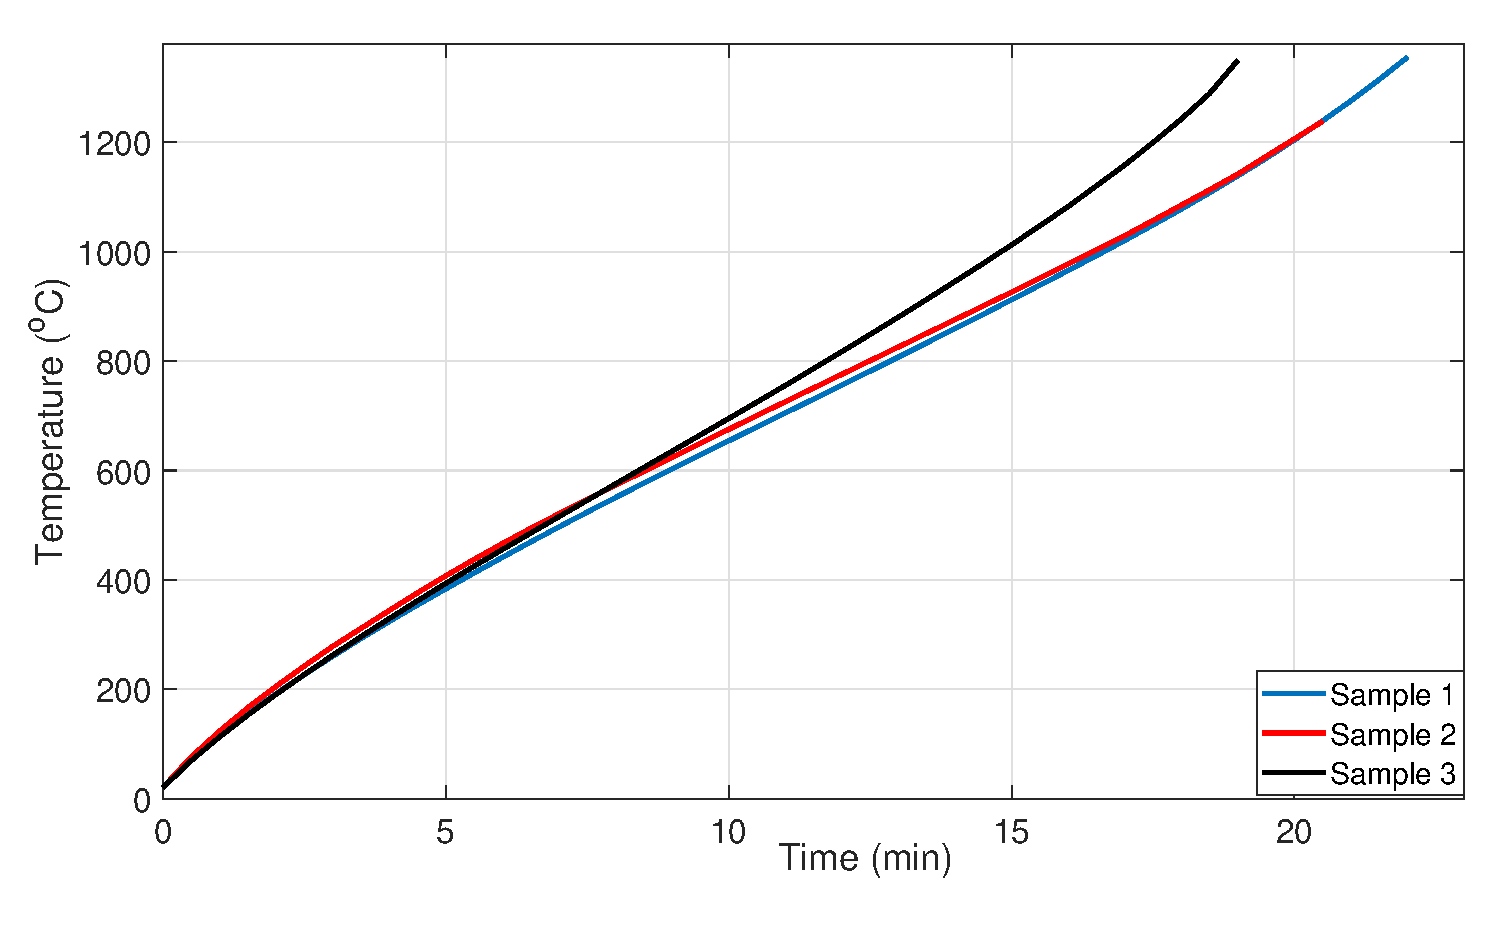
\includegraphics[width=1\linewidth]{2a.eps}
		\caption{Temperature of 3 samples in wind boxes.}
		\label{TempCurves}
	\end{subfigure}%
	\begin{subfigure}{.5\textwidth}
		\centering
		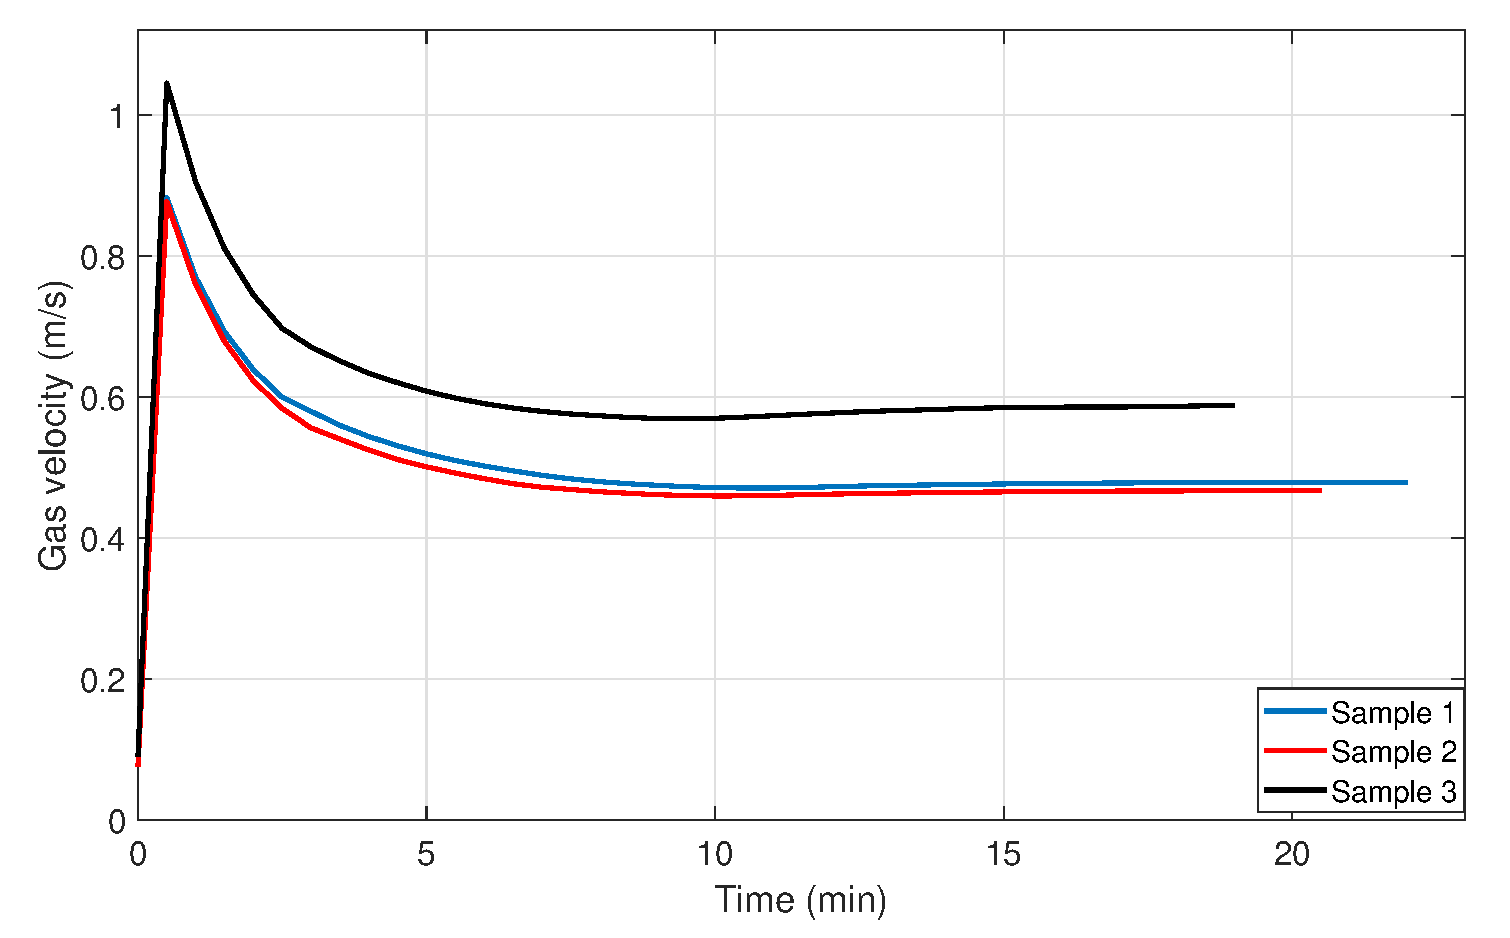
\includegraphics[width=1\linewidth]{2b.eps}
		\caption{Gas velocity of 3 samples in wind boxes.}
		\label{VelocCurves}
	\end{subfigure}
	\caption{Parameters for prediction.}
	\label{fig:PredictParams}
	\end{figure}

According to the literature, the gas velocity has an influence  on the charge temperature and could be determine through the pressure drop across the bed data $\Delta p$ , then the gas velocity $\nu$ (Fig.~\ref{VelocCurves}) in the lower part of charge can be calculated using Ergun equation:
\begin{equation} \label{eq:Ergun}
\frac{\Delta p}{L}=\frac{150\mu \nu(1-\varepsilon)^2}{d^2\varepsilon^3}+
\frac{1.75\rho \nu^2(1-\varepsilon)}{d\varepsilon^3}
\end{equation}
where $L [m]$ is the height of the bed, $\mu [Pa\cdot s]$ is the dynamic viscosity of gas, $\rho$ is the density of the charge, $\varepsilon$ is the porosity of porous matrix is calculated following \cite{Kaymak2017} and $d [m]$  is the equivalent particle size. 

\section{Determination of BTP grey model} \label{GreyModel}
Building a data  acquisition system with data storage, analysis and continuous retraining requires tremendous resources both in time and in finance. Also, the initial data collection, training and building an effective system requires constant interruption on the main production process, which affects on its effectiveness. In the considered production there is no data acquisition system, therefore, to obtain data, additional measurement systems were required that were not included in the main control loop. In such conditions, it becomes necessary to use models which requires a small amount of the initial sample to train and construct predictive model. The theory of grey systems satisfies these requirements.

Grey theory is a relatively new theory for prediction issues. One of the main characteristic of grey system theory is the accumulated generating operation (AGO), which is used to reduce randomness of the data. The mathematical relation of first-order AGO data (1-AGO) is described as following:

\begin{equation}
X^{(1)}(t)=\sum_{l=1}^{t}X^{(0)}(l),
Y^{(1)}(t)=\sum_{l=1}^{t}Y^{(0)}(l),
\end{equation}
where $X^{(0)}$, $Y^{(0)}$ are the original series and  $X^{(1)}$,  $Y^{(1)}$  are 1-AGO data.

Temperature in the wind boxes is considered as predicted series $Y$. The gas velocity $\nu$, calculated from the known pressure $\Delta p$ (from \eqref{eq:Ergun}), which is measured in real time was selected as an influencing factor $X$.

The influence of several factors on the predicted value for grey models can be considered only on the basis of model modifications GM(1,n), which is clearly demonstrated in the work \cite{Tien2008}. A continuous convolution integral grey model GMC(1,n) \cite{Kaymak2017} is one of the basic models with $(n-1)$ influencing factors. On the basis of this model, other continuous linear grey models with $(n-1)$ influencing factors were developed. For example, an interval model with a convolution integral IGDMC(1,n) \cite{Tien2008}, is intended for prediction of the interval of the variable. Model FGMC(1,n) \cite{Tien2011}  is developed on the basis of effectiveness of the first pair of original data. The deterministic grey model with the convolution integral DGDMC(1,n) \cite{Tien2009} distinguishes from GMC(1,n) by the estimation of first derivative and parameters: first derivative is estimated numerically by the cubic curve of the spline and the parameters of the model, according to the scheme of deterministic convergence. The error in the strength prediction considered by Tien is 0.54\% for FGMC(1,n), 1.25\% for GMC(1,n), 1.85\% for DGDMC(1,n) and 2.4\% for IGDMC(1,n). Later in \cite{Wang2014} was showed the optimized model GDMC(1,n) \cite{Tien2011} – OGDMC(1,n), in which the grey derivative value $dX_1^{(1)}(t)/dt$ is determined not by the weighted mean value $X_1^{(1)}(t)$ and $X_1^{(1)}(t-1)$,  but through the weight coefficient $\rho_i$, determined using the PSO algorithm \cite{Kennedy1995}:
\begin{equation}
\rho_iX_i^{(1)}(t)+(1-\rho_i)X_i^{(1)}(t)
\end{equation} 
\footnotetext{\textbf{Abbreviations:} GM, grey model; GMC, convolution integral grey model; FGMC, first-pair-of-data convolution integral grey model; IGDMC, interval grey dynamic model with convolution integral; DGDMC, deterministic grey dynamic model with convolution integral; OGDMC, optimized grey dynamic model with convolution integral }

Here, a value for the root mean squared percentage error to the priori sample period (RMSPEPR) in the OGDMC(1,n) decreased by 3.8 times – from 7.07\% to 1.86\%.
To select the most accurate model for predicting the BTP in the wind box, we will conduct experiments using models FGMC(1,n), GMC(1,n) and OGDMC(1,n), which have the lowest prediction error value.

\subsection{GMC(1,n)}

The gas velocity, calculated from the known pressure $\Delta p$, which is measured in real time was selected as an influencing factor. Convolution integral grey model GMC(1,2) with one influencing factor is a linear differential model:
\begin{equation} 
\frac{dY^{(1)}(t)}{dt}+b_1Y^{(1)}(t)=b_2X^{(1)}(t)+u \label{diffEq}
\end{equation}
The grey derivative for the first-order AGO data in \eqref{diffEq} is conventionally represented as:
\begin{equation} 
\frac{dY^{(1)}(t)}{dt}=\lim\limits_{\Delta t\to \infty}\frac{Y^{(1)}(t+\Delta t)-Y^{(1)}(t)}{\Delta t}
=Y^{(1)}(t+\Delta t)-Y^{(1)}(t)
\end{equation}
when $\Delta t \to 1$. The parameters of \eqref{diffEq} are determined by least square method:
\begin{equation} \label{eq:LSM}
[b_1,b_2,u]^T = (B^TB)^{-1}B^TY_R
\end{equation}
where $t$  changes from $1$ to $r$  which is the number of initial sample to construct the model in \eqref{diffEq},
\begin{equation} \label{eq:Bmatrix}
B = \begin{bmatrix}
-0.5\left(Y^{(1)}(1)+Y^{(1)}(2)\right) & 0.5\left(X^{(1)}(1)+X^{(1)}(2)\right) & 1 \\ 
-0.5\left(Y^{(1)}(2)+Y^{(1)}(3)\right) & 0.5\left(X^{(1)}(2)+X^{(1)}(3)\right) & 1 \\
. & . & .\\
-0.5\left(Y^{(1)}(r-1)+Y^{(1)}(r)\right) & 0.5\left(X^{(1)}(r-1)+X^{(1)}(r)\right) & 1
\end{bmatrix}
\end{equation}

\begin{equation}
Y_R = [Y^{(1)}(2),Y^{(1)}(3),...,Y^{(1)}(r)]^T
\end{equation}

Prediction of the sinter temperature $\hat{Y}^{(0)}$ is:
\begin{equation} \label{eq:Yhat}
\hat{Y}^{(0)}(t) = \hat{Y}^{(1)}(t)-\hat{Y}^{(1)}(t-1)
\end{equation}
where
$\hat{Y}^{(1)}(t)=Y^{(0)}(1)e^{-b_1(t-1)} + \frac{1}{2}e^{-b_1(t-1)}
\times\left(b_2X^{(1)}(t)+u\right) +\frac{1}{2}\left(b_2X^{(1)}(t)+u\right) 
+\sum_{i=2}^{t-1}e^{-b_1(t-i)}\left(b_2X^{(1)}(i)+u\right)$

\subsection{FGMC(1,n)}

The differential equation of grey prediction model FGMC(1,n) presented in \cite{Tien2011} is the same as for GMC(1,n), but modeled with data including the information from the first pair of original data. The parameters of \eqref{diffEq} are determined using the LSM \eqref{eq:LSM}, where 
\begin{equation}
B = \begin{bmatrix}
-0.5\left(Y^{(1)}(0)+Y^{(1)}(1)\right) & 0.5\left(X^{(1)}(0)+X^{(1)}(1)\right) & 1 \\ 
-0.5\left(Y^{(1)}(1)+Y^{(1)}(2)\right) & 0.5\left(X^{(1)}(1)+X^{(1)}(2)\right) & 1 \\
. & . & .\\
-0.5\left(Y^{(1)}(r-1)+Y^{(1)}(r)\right) & 0.5\left(X^{(1)}(r-1)+X^{(1)}(r)\right) & 1
\end{bmatrix}
\end{equation}
\begin{equation} \label{eq:YR}
Y_R = [Y^{(1)}(1),Y^{(1)}(2),...,Y^{(1)}(r)]^T
\end{equation}

Prediction of the sinter temperature is:
\begin{equation}
\hat{Y}^{(0)}(t)=Y^{(0)}(0)e^{-b_1t}+u(t-1) \times\sum_{i=1}^{t}\left(\frac{1}{2}e^{-b_1(t-i+0.5)}b_2\left(X^{(1)}(i)-X^{(1)}(i-1)\right)\right)
\end{equation}

\subsection{OGDMC(1,n)}

Differential equation of the Grey dynamic model with convolution integral is:
\begin{equation} \label{eq:OGDMC}
\frac{dY^{(1)}(t)}{dt}+b_1Y^{(1)}(t)
=b_2+\sum_{i=2}^{n}\left(b_{2i-1}\frac{dX^{(1)}(t)}{dt}+b_{2i}X^{(1)}(t)\right)
\end{equation}

The parameters of \eqref{eq:OGDMC} are determined using the LSM \eqref{eq:LSM}, the vector $Y_R$ is calculated according to \eqref{eq:YR} and
\begin{equation}
B = \begin{bmatrix}
-0.5\left(Y^{(1)}(1)+Y^{(1)}(2)\right) &1&X^{(0)}(1)& 0.5\left(X^{(1)}(1)+X^{(1)}(2)\right)   \\ 
-0.5\left(Y^{(1)}(2)+Y^{(1)}(3)\right) &1&X^{(0)}(2)&  0.5\left(X^{(1)}(2)+X^{(1)}(3)\right) \\
. & . & . & .\\
-0.5\left(Y^{(1)}(r-1)+Y^{(1)}(r)\right)&1&X^{(0)}(r)&  0.5\left(X^{(1)}(r-1)+X^{(1)}(r)\right) 
\end{bmatrix}
\end{equation}

Prediction of the temperature is determined by \eqref{eq:Yhat}, where:
\begin{align}
\hat{Y}^{(1)}(t)=Y^{(0)}(1)e^{-b_1(t-1)} + u(t-2) \times  \sum_{\tau=2}^{t}(\frac{1}{2}e^{-b_1(t+0.5-\tau+0.5\lambda_1)}\times
[0.5\left( f(\tau)+f(\tau-1) \right) + \nonumber\\
+0.5\lambda_1\left( f(\tau)+f(\tau-1) \right) ]+\frac{1}{2}e^{-b_1(t+0.5-\tau+0.5\lambda_2)}
\times[0.5\left( f(\tau)+f(\tau-1) \right) + 0.5\lambda_2\left( f(\tau)+f(\tau-1) \right) ]  )\
\end{align}
where $\lambda_1 = -1/\sqrt{3}$, $\lambda_2 = 1/\sqrt{3}$ and
$
f(t) = b_2 + \sum_{i=2}^{n}\left(b_{2i-1}X^{(0)}(t)+b_{2i}X^{(1)}(t)\right)
$

\subsection{Size of samples to construct the model}
The number of data to construct a predictive model is an important parameter, which leads to reduce the error in temperature prediction. Also it allows to define wind boxes, where thermocouples should be installed in the future and reduce their quantity for economy. The main feature of grey theory is its capability to use as few as $n+3$ pairs of data by GMC(1,n) \cite{Tien2005}. For each sample, the following experiments were performed: (1) based on the n-pair of series from the sample, the model was built, (2)	based on the model, the prediction of the remaining values was made, (3) the prediction results were compared to the original samples and the Root Mean Squared Percentage Error (RMSPE) according to \eqref{eq:RMSPE} was calculated.
\begin{equation} \label{eq:RMSPE}
RMSPE = \sqrt{\frac{1}{n}\sum_{i}\frac{\left(\hat{Y}_i-Y_i\right)^2}{Y_i^2}}\times 100\%
\end{equation}
During the experiments, 17 models were built for each sample ranging from 5 to 20 pair of series. The results of the predicted errors for each sample are presented in Fig.~\ref{fig:RMSPE}.
The predicted errors for each sample take the minimum values for different pairs of series, ranging from 14 to 17 pair of series. The mean smallest predictive error for 3 samples is achieved with 15 pair of series.

\subsection{BTP prediction results for considered models}
The RMSPE for the post sample period of predictive models for 3 samples (Fig. \ref{TempCurves}) are presented in the Table~\ref{tab:RMSPE1}, where the volume of initial sample $r$  to construct the model includes data from the beginning of sintering process up to 7.5 min (15 values). Results of predictive models for sample 1 are shown in Fig.~\ref{fig:GMsSample1} and RMSPE of all samples are presented in Table \ref{tab:RMSPE1}. The best result for predicting the BTP of the charge was obtained as a result of using the GMC(1,n) model.  

The predictive results based on grey systems do not improve the accuracy in comparison with the other models, but allow to build an adequate prediction model of BTP in the absence of a large amount of historical temperature data. Additional advantage is the time saving for data collection and model training. 

\begin{center}
	\begin{table}[t]
		\centering
		\caption{RMSPE of grey models, \%} \label{tab:RMSPE1}
		\begin{tabular*}{500pt}{@{\extracolsep\fill}cccc@{\extracolsep\fill}}
			\toprule
			\textbf{No of sample} & \textbf{\textit{GMC(1,n)}}& \textbf{\textit{FGMC(1,n)}}& \textbf{\textit{OGDMC(1,n)}} \\
			\midrule
			1 & 2.2413 & 4.1062 & 2.6575 \\
			2 & 1.6697 & 3.4544 & 3.6921 \\
			3 & 1.0952 & 3.8123 & 4.1833 \\
			\bottomrule
		\end{tabular*}
	\end{table}
\end{center}
\begin{figure}
	\centering
	\parbox{8.5cm}{
		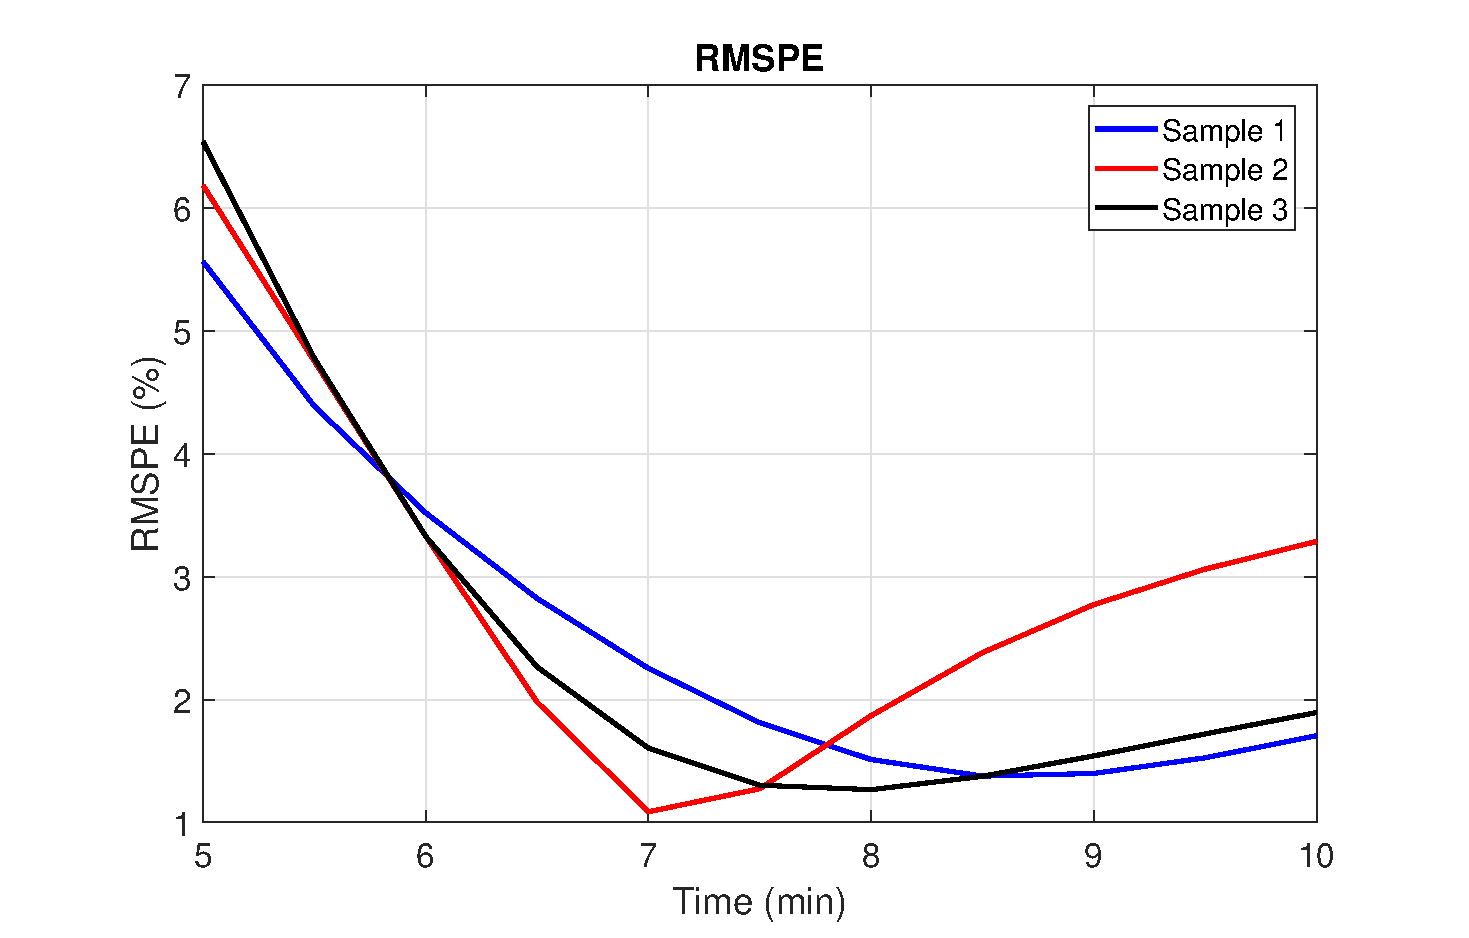
\includegraphics[width=8.5cm]{3.eps}
		\caption{Predictive errors depending on sample sizes.}
		\label{fig:RMSPE}}
	\qquad
	\begin{minipage}{8.5cm}
		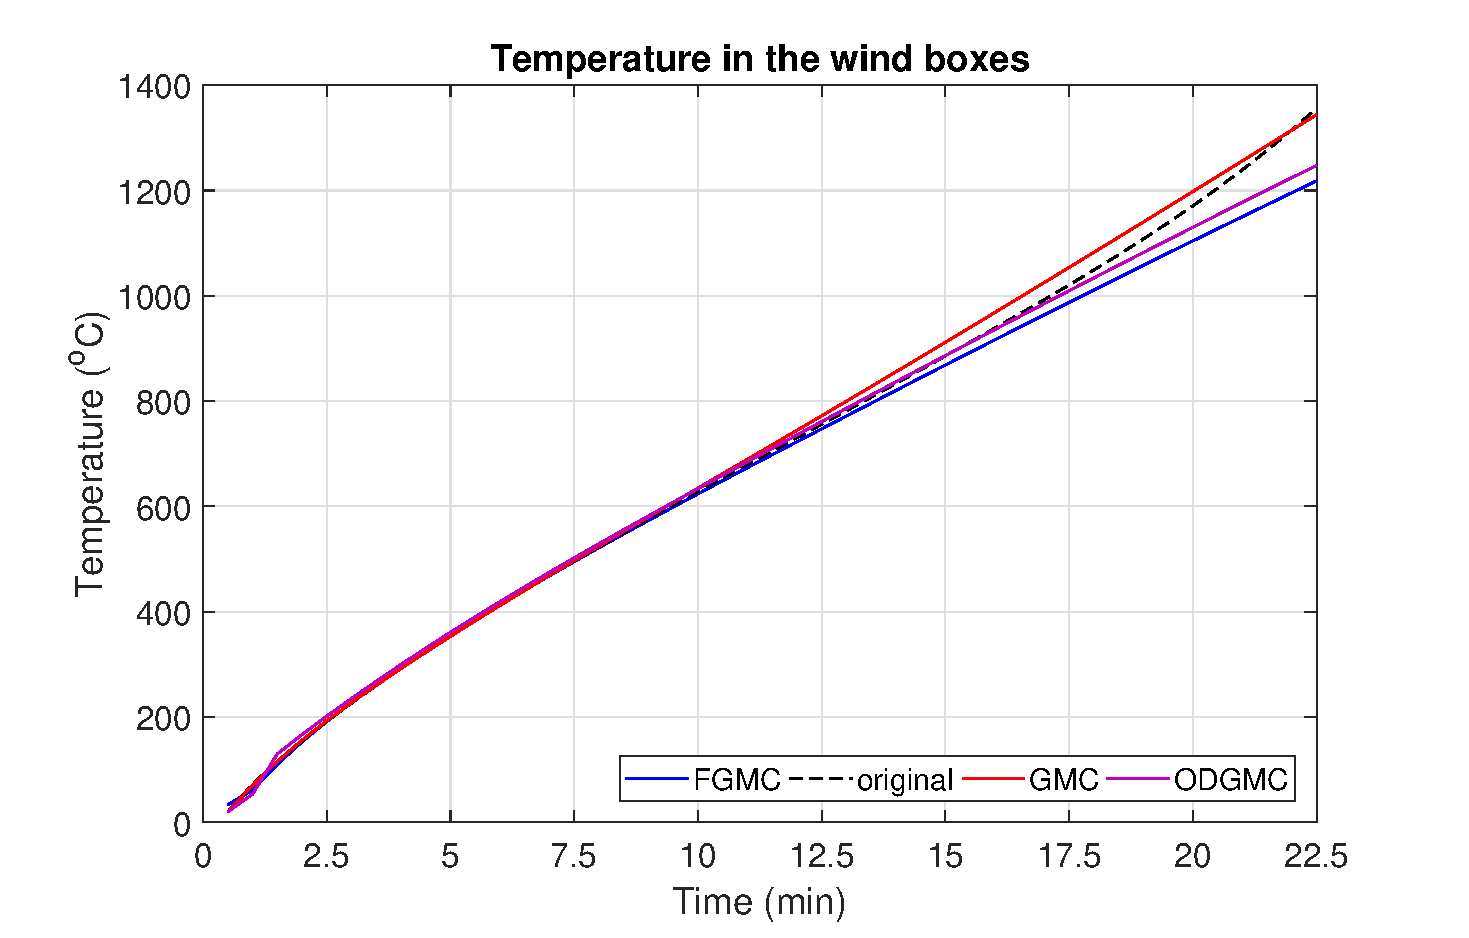
\includegraphics[width=8.5cm]{4.eps}
		\caption{Modeling results of sample 1}
		\label{fig:GMsSample1}
	\end{minipage}
\end{figure}
	
\subsection{Optimal GMC(1,n)}
To improve the accuracy of the predictive model GMC(1,n) instead of the weighted mean to determine the grey derivative, we introduce the coefficient $\rho \in [0;1]$, then \eqref{eq:Bmatrix} takes the following  form:
\begin{equation}
B = \begin{bmatrix}
-(1-\rho)Y^{(1)}(1)+\rho Y^{(1)}(2) & (1-\rho)X^{(1)}(1)+\rho X^{(1)}(2) & 1 \\ 
-(1-\rho)Y^{(1)}(2)+\rho Y^{(1)}(3) & (1-\rho)X^{(1)}(2)+\rho X^{(1)}(3) & 1 \\
. & . & .\\
-(1-\rho)Y^{(1)}(r-1)+\rho Y^{(1)}(r) &(1-\rho)X^{(1)}(r-1)+\rho X^{(1)}(r) & 1
\end{bmatrix}
\end{equation}

Coefficient $\rho$ is determined by a PSO method \cite{Kennedy1995}. This algorithm is a system of particles that move to optimal solutions, each particle contains the coordinates of the found best solution ($pbest$) and the best solution from all the particles in the swarm ($gbest$). The direction and length of the particle velocity vector is determined by the following formula:
\begin{equation} \label{PSO}
\upsilon_i = \upsilon_i + a_1rnd()\cdot (pbest_i-x_i)+a_2rnd()\cdot(gbest_i-x_i)
\end{equation}
where $\upsilon_i$  is the particle speed vector, $a_1, a_2$   are the constant accelerations and $x$  is the particle current position. In this case the particle current position is the coefficient $\rho$. As an optimality criterion, the minimum of the \eqref{eq:RMSPE} is used. The obtained predictive models and the RMSPE for the post sample period are presented in Table \ref{tab:OGMC}, where it can be seen that the accuracy of the grey model is improved.

In \cite{Wang2014}, interpolation coefficients $\rho_i$ are introduced into the background values of each of the variables in GDMC(1,n). Application of this algorithm to GMC(1,n) model will have the following changes in \eqref{eq:Bmatrix}:

\begin{equation}
B = \begin{bmatrix}
-(1-\rho_1)Y^{(1)}(1)+\rho_1 Y^{(1)}(2) & (1-\rho_2)X^{(1)}(1)+\rho_2 X^{(1)}(2) & 1 \\ 
-(1-\rho_1)Y^{(1)}(2)+\rho_1 Y^{(1)}(3) & (1-\rho_2)X^{(1)}(2)+\rho_2 X^{(1)}(3) & 1 \\
. & . & .\\
-(1-\rho_1)Y^{(1)}(r-1)+\rho_1 Y^{(1)}(r) &(1-\rho_2)X^{(1)}(r-1)+\rho_2 X^{(1)}(r) & 1
\end{bmatrix}
\end{equation}

The predictive results have changed slightly (Table \ref{tab:OGMC}), but the time to find the optimal values of the $rho_i$ increased. Increase of $(n-1)$ dependent variables leads to increase optimization time exponentially and to a difficulty of using the algorithm with different coefficients for each variable in real-time control. Therefore to enhance the modelling and predictive accuracy one coefficient $\rho$ is used to control task.

The coefficients of grey model (Table \ref{tab:OGMC}), which were found by \eqref{eq:LSM}, are differ significantly for each sample. This is due to the fact that each temperature curve was obtained under different initial conditions. Moreover, in production under real conditions, it is not possible to continuously control the composition of the charge. Therefore, it is necessary to build a predictive model, which uses only measured real time factors and dynamically constructs the model for a certain batch of sintered ore. 

\begin{table}[htbp]
	\caption{Results of optimal GMC(1,n) model}
	\begin{center}
		\begin{tabular*}{500pt}{@{\extracolsep\fill}ccccccc@{\extracolsep\fill}}
			\toprule
			\textbf{No} & \textbf{GMC (1,n) type} &\textbf{$\rho$} & \textbf{$b_1$}  & \textbf{$b_2$} &\textbf{$u$} & \textbf{RMSPE, \%}\\
			\midrule
			1&GMC (1,n), $\rho$& 0.2261 & -0.0005 & 56.3769 & 28.3447 & 1.2120 \\
			&GMC (1,n), $\rho_i$ & 0 \& 0.2283 & -0.0005 & 56.3554 & 28.4573 & 1.2110 \\
			\midrule
			2& GMC (1,n), $\rho$ & 0.3669 & 0.0003 & 58.9057 & 30.6943 & 1.4266 \\
			&GMC (1,n), $\rho_i$ & 1 \& 0.3683 & 0.0003 & 58.8892 & 30.7584 & 1.4249 \\
			\midrule
			3&GMC (1,n), $\rho$& 0.4193 & 0.0025 & 62.1686 & 37.5064 & 0.9756 \\		
			&GMC (1,n), $\rho_i$ & 1 \& 0.4384 & 0.0023 & 61.9513 & 38.5224 & 0.9588 \\
			\bottomrule
		\end{tabular*}
		\label{tab:OGMC}
	\end{center}
\end{table}
\section{Control structure} \label{ControlStruct}
Dynamic construction of the grey model uses only actual data, which represent real time information about sintering process, not depends on historical data and will make possible to obtain the prediction of the charge temperature. If the predictive temperature of the charge at the end of the strand does not reach the set point (the highest temperature in the wind boxes), then it is necessary to control the sinter process. The control can be carried out by changing the amount of fuel in the initial charge, the strand speed and the underpressure created in the wind boxes. The change in the amount of fuel affects only the charge that has not yet been fed to the sinter, so this effect is not considered in the work.

The idea to build the prediction model of the BTP in real time was also considered in \cite{Wu2012a}, where the model parameters are determined by the closed-loop identification method. High accuracy of the generalized prediction model \cite{Wu2012a} was achieved by a real-time measurement of additional parameters, which makes the proposed model more expensive.

The proposed control structure for the BTP is presented in the Fig.~\ref{fig:ControlStructure} and has the following algorithm:  after the charge is passed under the horn, the system begins collecting data on temperature, pressure in the wind boxes and sinter machine speed. Based on the collected data, a forecast model is built on the basis of the grey model that predicts the temperature at the end of the sintering machine. If the temperature does not correspond to the BTP, a predictive optimization algorithm calculates the necessary values of the sinter speed and pressure in the wind boxes. The resulting values are fed to the appropriate controllers. After charge is reaching the end of sintering machine, the cycle is repeated for the next charge. 
\begin{figure}[htbp]
	\centering
	\resizebox{11 cm}{!}{
		\includegraphics{5.png}}
	\caption{Control structure for the BTP.} \label{fig:ControlStructure}
\end{figure}

The PSO is used as a method of predictive optimization. Its distinguishing feature from many other methods is that, for the particle swarm method, we can calculate only the value of the function being optimized, but not its gradient. In terms of efficiency, it can compete with other methods of global optimization, and its low algorithmic complexity contributes to the simplicity of its implementation. 
Particle current position \eqref{PSO} includes two variables: number of samples that represents time of sinter process and gas velocity.

The PSO algorithm is composed of the following steps: 

(1) Generate $m$-particles ($m=2$) in the $n$-dimensional space. Position and velocity are represented by $x_i=(x_{i1},x_{i2},..,x_{in})$ and $\upsilon_i = (\upsilon_{i1},\upsilon_{i2},..,\upsilon_{in})$, $i=1,..,m$. 

(2) Generate randomly the initial position of the particles $x_i$ within the limits $t_{min} \leqslant x_1 \leqslant t_{max}$, $X_{min} \leqslant x_2 \leqslant X_{max}$ and initial velocity vector $\upsilon_{i}$. $t$ is the time step and $X$  is the underpressure in the wind boxes. 

(3) According to \eqref{eq:LSM} substitute $x_2$ into the matrix $B$ and according to \eqref{eq:Yhat} put $x_1$ as parameter $t$. 

(4) Calculate the fitness value \eqref{eq:RMSPE} for each particle.

(5) Compare each particle’s fitness to the global best position $pbest$ to adapt to the value; if it is the optimum, it can be taken as the best position; if not, turn to next step.

(6) Update particles velocity and position according to the evolution equation \eqref{PSO}.

(7) If stopping criteria are met, show the output and its fitness, which corresponds to the optimal parameters and the RMSPE, or else go back to step 3.

With the help of the obtained optimal sintering process time $t$  value, the strand speed is determined, and through the optimum gas velocity value, the underpressure in wind boxes is found according to \eqref{eq:Ergun}. Modeling results using the BTP control system for the samples are represented in Fig.~\ref{fig:ControlResults}. In the first sample, the sintering temperature of the charge is reached in 22 minutes. To increase line productivity, extended boundaries of inequalities are set. Wherein, the optimization algorithm allows to find such values of strand speed and pressure in wind boxes at which the BTP is reached in 19.5 minutes. The sample 1 results of forecast optimization are follows: the speed values change from 3.5 m/min to 4.5 m/min and the pressure in wind boxes from 800 mmHg to 760 mmHg. In the second sample, the BTP is not reached. Therefore, as a result of predictive optimization, a new value is supplied to the pressure regulator, at which the sintering temperature is reached. In the third case, as a result of predictive optimization, the speed of sinter strand and pressure in wind boxes are increased, which allows to achieve the optimum temperature in 19 min.

\begin{figure}
	\centering
	\begin{subfigure}{.5\textwidth}
		\centering
		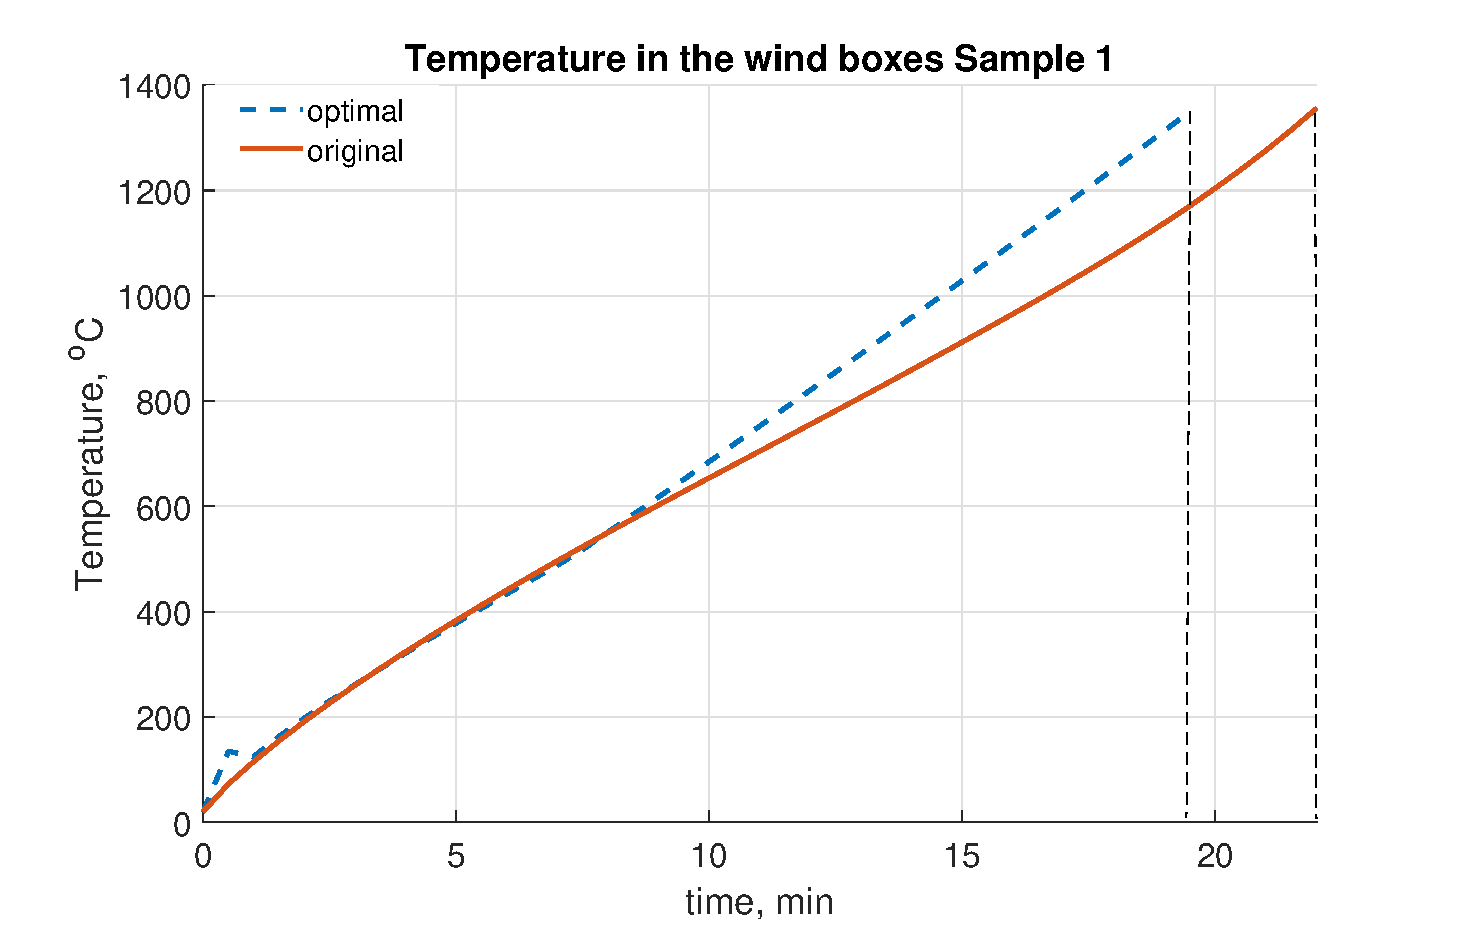
\includegraphics[width=1\linewidth]{6a.eps}
	\end{subfigure}%
	\begin{subfigure}{.5\textwidth}
		\centering
		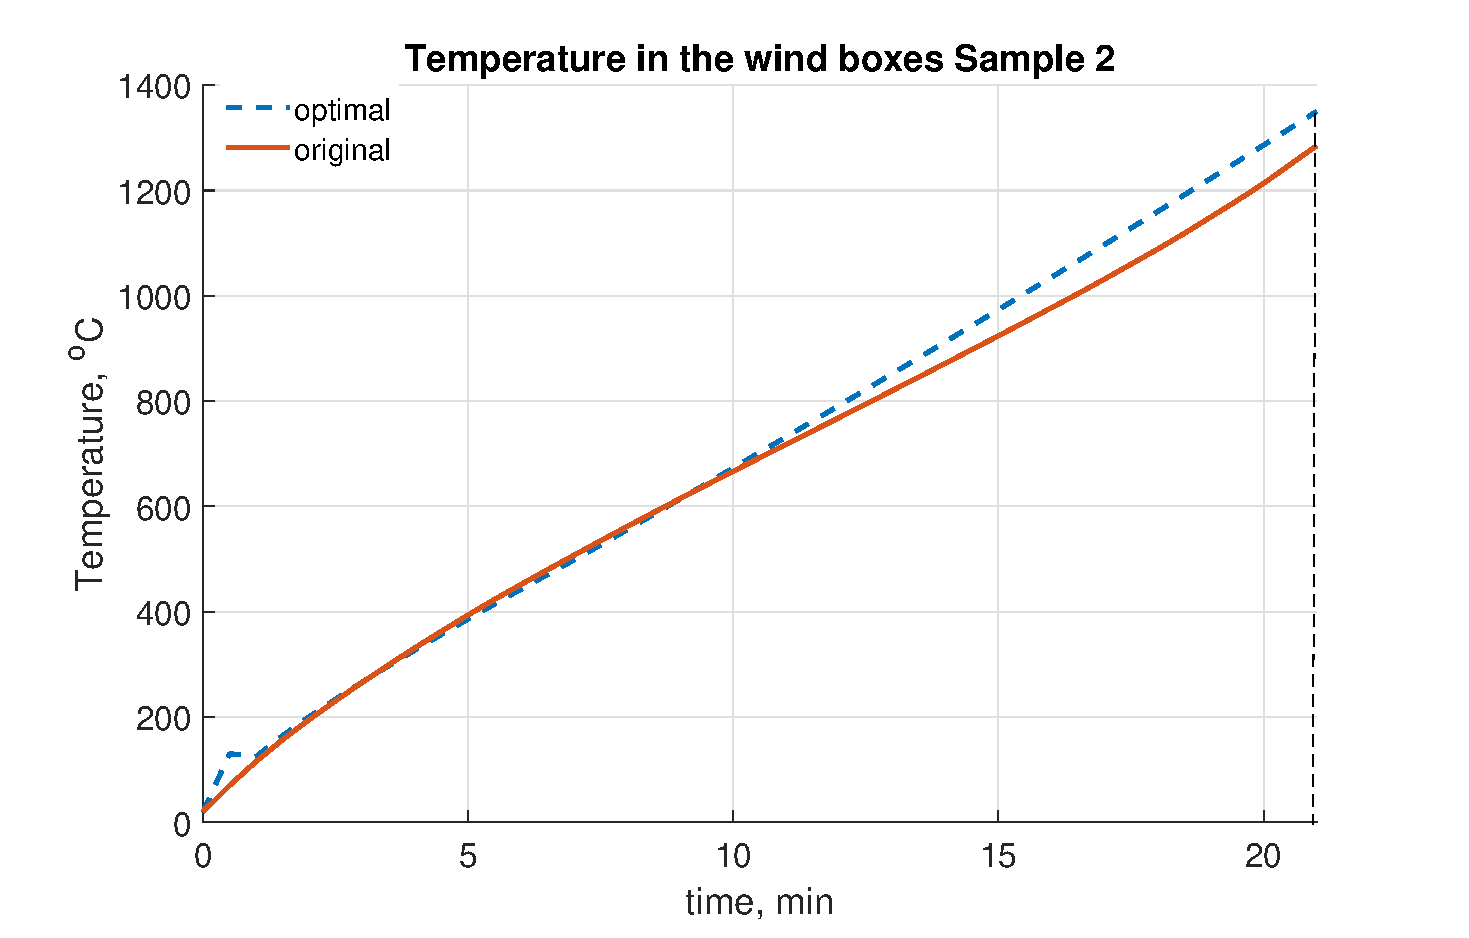
\includegraphics[width=1\linewidth]{6b.eps}
	\end{subfigure}
	\begin{subfigure}{.5\textwidth}
	\centering
	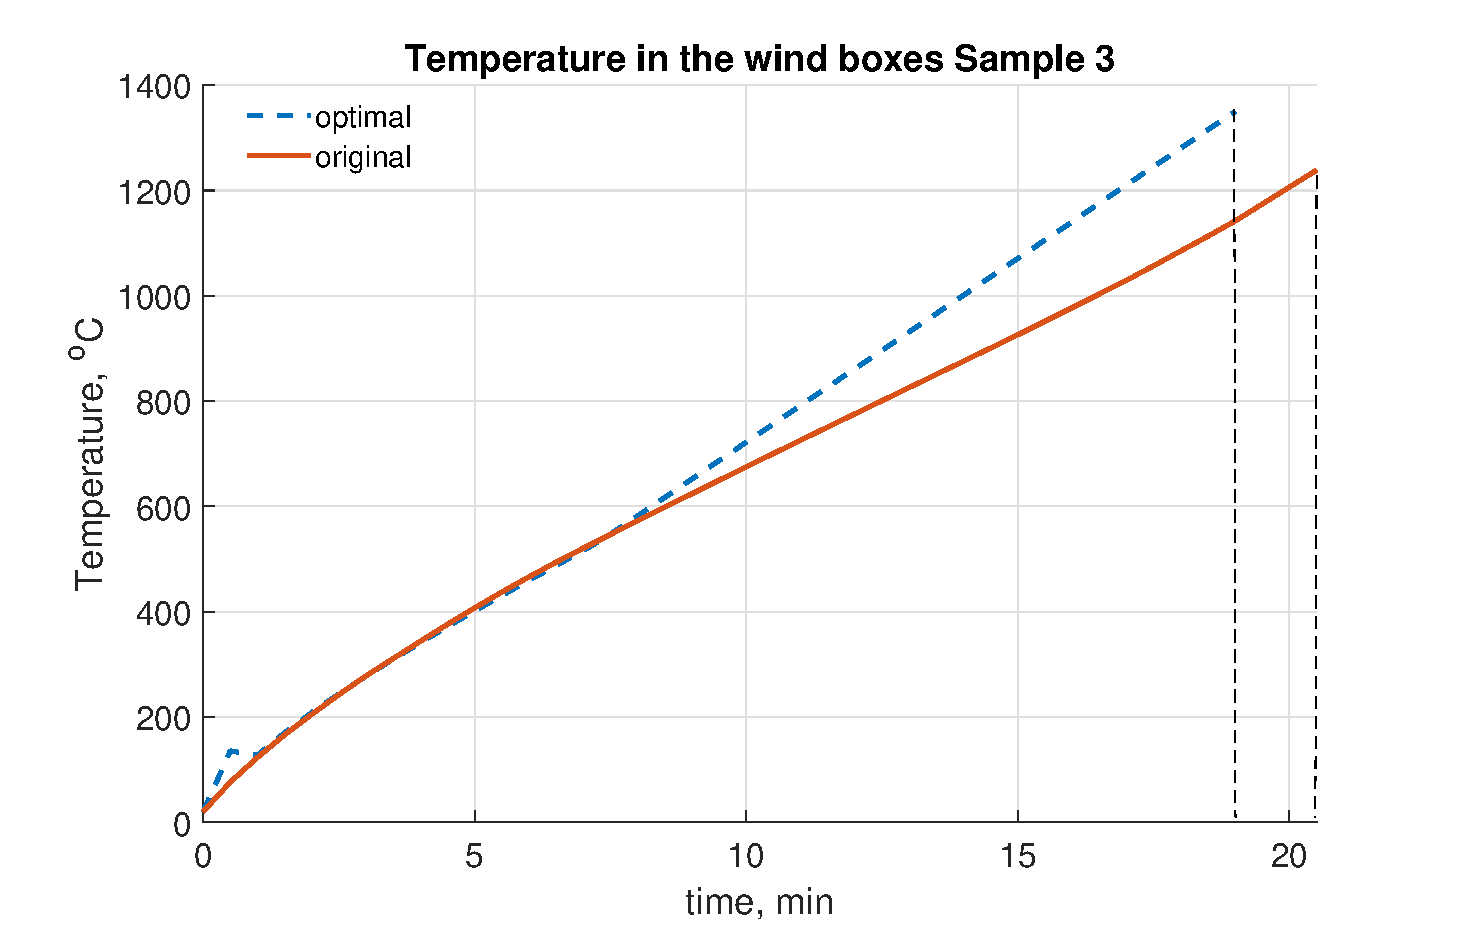
\includegraphics[width=1\linewidth]{6c.eps}
	\end{subfigure}
	\caption{Modeling results of the BTP using the control structure.}
	\label{fig:ControlResults}
\end{figure}
\section{Conclusions} \label{Conclusion}
The proposed control process structure of phosphorite ore sintering considered in this paper is intended to improve the product quality and reduce the return. As an indicator responsible of the sintering quality, the BTP was chosen, i.e. the position at which the process reaches the highest temperature. Prediction of this variable was realized through the grey predictive model with some main contributions: (1) dynamic construction of the predictive model using a small samples size, obtained from the beginning of the process, which reduces the time for data acquisition and system training; (2) control of the sintering process not only based on the strand speed, but also on the underpressure in the wind boxes; (3) use of a grey model with (n-1) influencing factors that takes into account not only the effect of the predicted value, but also other process variables; (4) modeling different continuous grey models and development of optimal GMC(1,n) model; (5) use of predictive optimization algorithm to determine optimal process parameters. In the framework of this article, the initial amount of data for constructing the model was also determined, as a result of which the amount of costs for building the data acquisition system is reduced, while the predictive model error does not exceed 1.5\%.
In future works, modeling and prediction results of the BTP using the control structure will be verified with industrial data, the proposed control structure will be applied on the industrial process in Kazakhstan, with  hardware, communication and  software including all real-time delays and noises from aquisition system. Moreover, in engineering applications, the BTP control is a part of the control of sinter quality, and our future research will focus on the combination of such control approach with other control parts, such as ignition control or water and coke quantity control.
\nocite{*}
\bibliography{wileyNJD-AMS}
\section*{Author Biography}

\begin{biography}{\includegraphics[width=60pt,height=70pt]{7.jpg}}{\textbf{Nigina Toktassynova.} Master of technical science, is currently a PhD student of Automation and Control specialty at the Satbayev University, Almaty, Kazakhstan. She earned her bachelor and master’s degree in automation and control at the Almaty university of power engineering and telecommunication, Almaty, Kazakhstan, in 2012, and 2014, respectively. Her research interests include predicitive algorithm, grey system theory and control systems in sintering process. }
\end{biography}
\begin{biography}{\includegraphics[width=60pt,height=70pt]{8.jpg}}{\textbf{Hassen Fourati.} PhD, is currently an associate professor of the electrical engineering and computer science at the University of Grenoble Alpes, Grenoble, France, and a member of the Dynamics and Control of Networks Team (DANCE), affiliated to the Pôle Automatique et Diagnostic (PAD) of the GIPSA-Lab. He earned his bachelor of engineering degree in electrical engineering at the National Engineering School of Sfax (ENIS), Tunisia; master’s degree in automated systems and control at the University of Claude Bernard (UCBL), Lyon, France; and PhD degree in automatic control at the University of Strasbourg, France, in 2006, 2007, and 2010, respectively. His research interests include nonlinear filtering, estimation and multisensor fusion with applications in navigation, motion analysis, mobility and traffic management.}
\end{biography}
\begin{biography}{\includegraphics[width=60pt,height=70pt]{9.jpg}}{\textbf{Batyrbek Suleimenov.} Doctor of Technical Science, is currently Head of Automation and Control Department and professor in Satbayev University, Almaty, Kazakhstan and a member of international engineering academy of Kazakhstan. He has 6 patents, more than 200 publications. His research interests include intelligent control systems for technological processes and systems for operational diagnostics of technological equipment.}
\end{biography}
\end{document}
